\noindent Previous cellular-scale modelling studies consider blood flow in simple geometries like long and uniform circular cross-sectional branches or in some instances complex geometries like vascular networks. The geometrically complex branching network of micro-vessels in large-scale micro-circulations pose a great challenge for researchers to model and reconstruct these vascular networks. The complex architecture of vascular networks is often characterised by bifurcating, merging and winding vessels.\cite{fung2013biomechanics} On top of this, different organs have different types of network topology. For example, blood vessels in the retina and kidney have a tree-like topology\cite{LiYiwen2008Dlav} while vessels in muscles form arcade-type planar networks\cite{KianiM1994Fimb, tawfik2013mathematical}(see Figure \ref{BloodNetworkTopology} for illustrations). For tumours, the blood vessels can have trifurcations and short-length shunts which further increases the complexity of the network.\cite{TumorMicrovasculature} Therefore, these geometrical differences can cause significant deviations in the haemodynamics of long straight branches compared to a vascular network.

\begin{figure}[H]
\centering
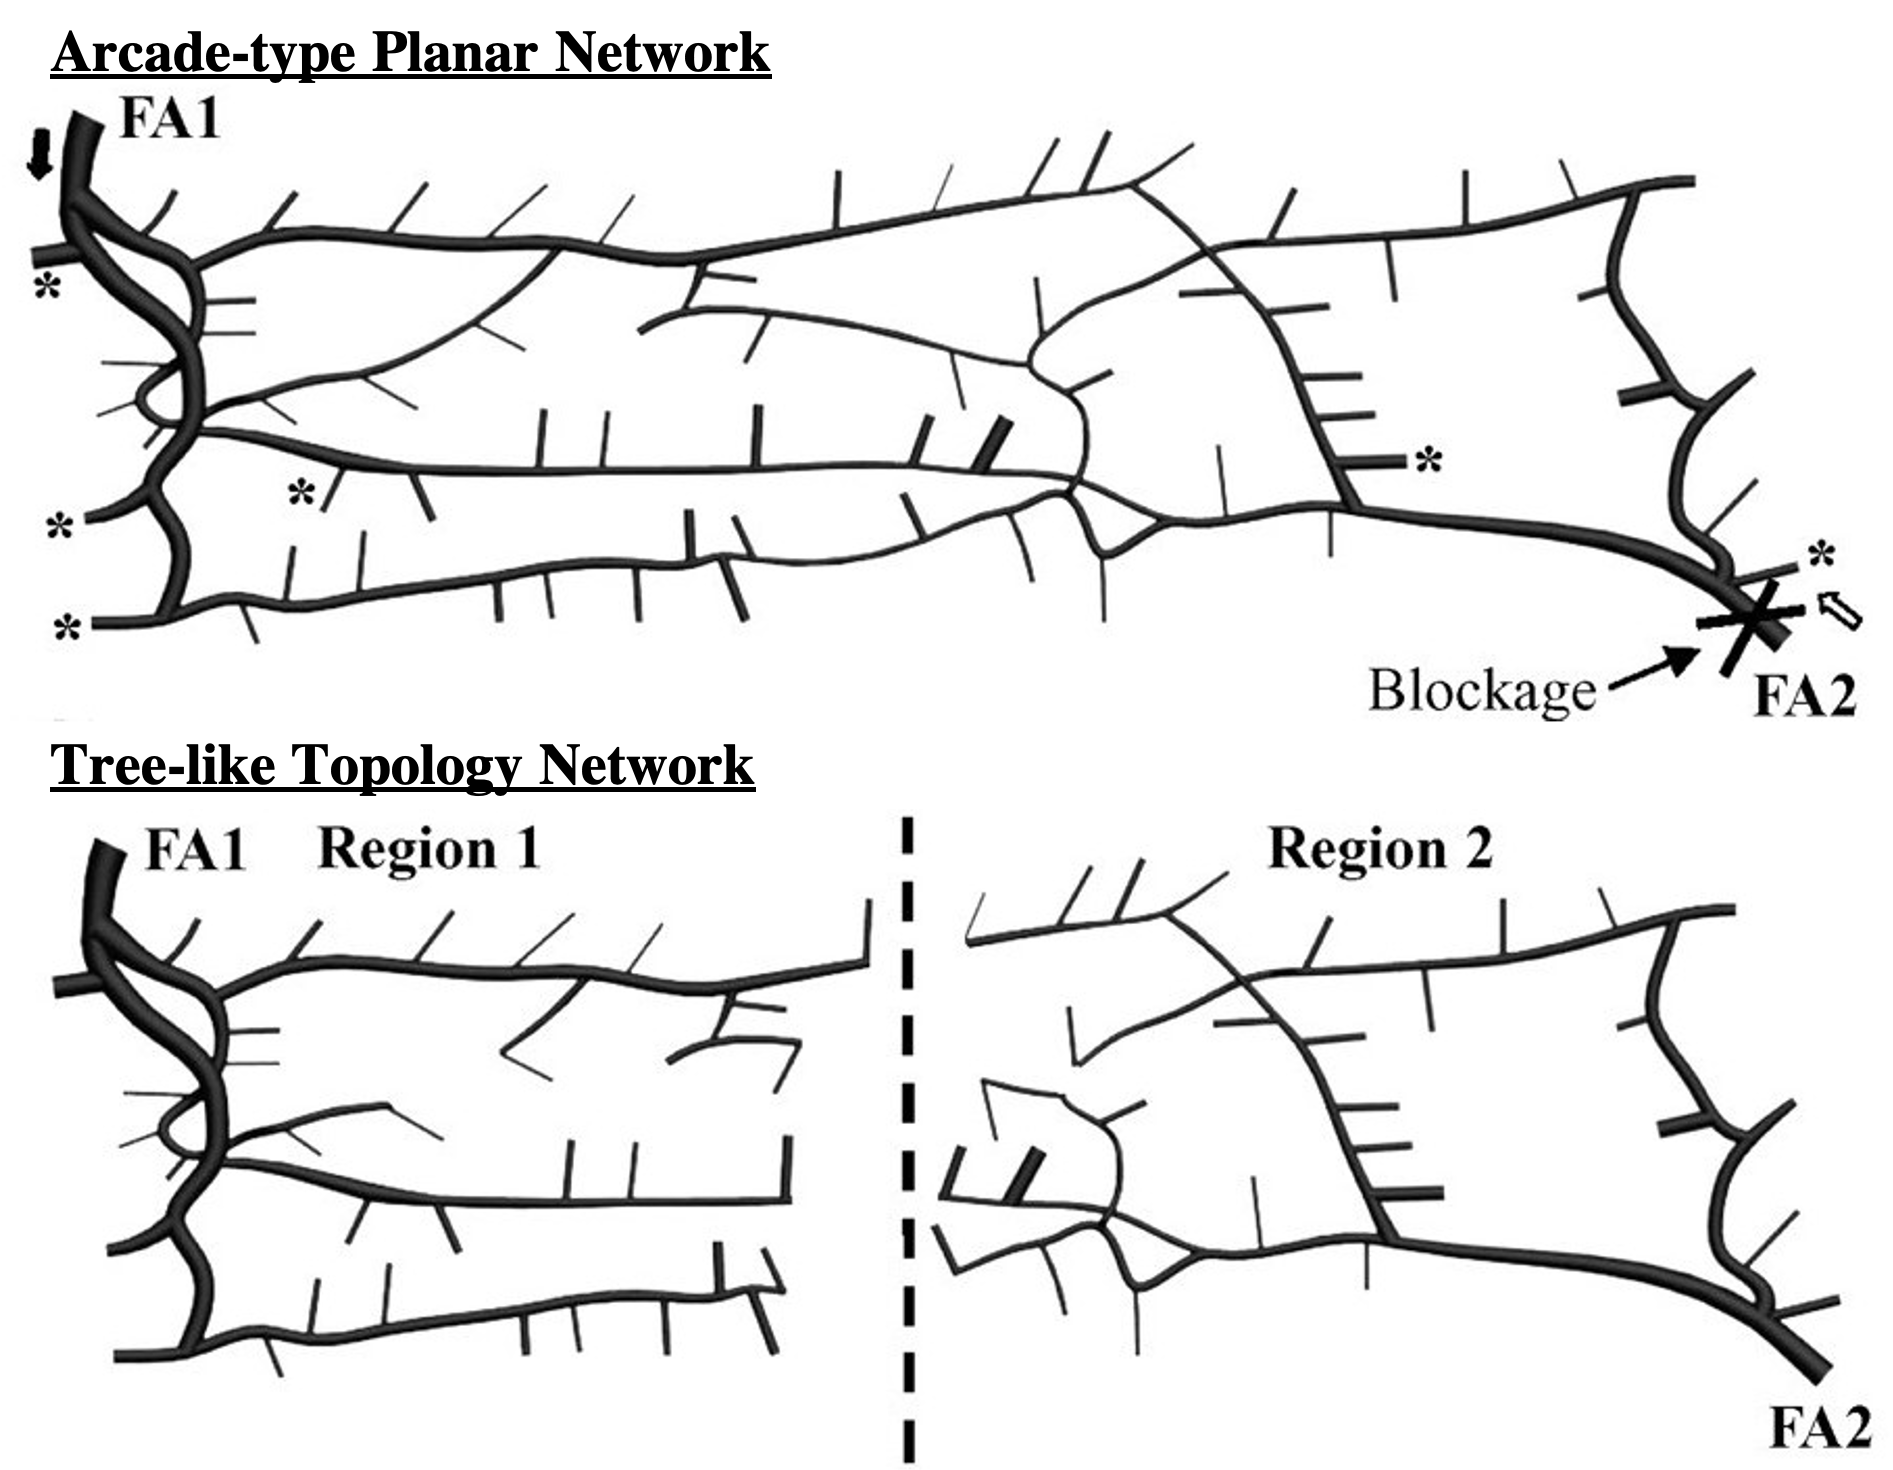
\includegraphics[width=0.6\textwidth]{images/TopologyNetworks.png}
\caption{\textit{Computer visualisation of an arcade-type and two-tree blood flow networks.\cite{NetworkTopology2005} FA1 and FA2 represent the branches of feed arteries with arrows indicating the direction of flow. Arcade outflows are shown with an asterisk (*) and all other open-end vessels are transverse arterioles.} \label{BloodNetworkTopology}}
\end{figure}

\subsubsection{2D \& 3D Simple Networks}
\noindent In general, most of the cellular-scale modelling studies conducted were investigating in either two- dimensional (2D) or three-dimensional (3D) computational simulations where the geometry of the networks were either idealised or obtained from the reconstruction of \textit{in vivo} images.\cite{PriesAR1990BFiM, reichold2011cerebral, Gould2015HematocritNetworks, Balogh2018, CharlesPhDThesis2020} However, there are considerable differences between both dimensional approaches. For example, there is a significant size difference between 3D to 2D translations because the RBC takes up more cross-sectional space in a 2D environment compared to 3D. Furthermore, using 2D models to replicate data from 3D realistic systems would neglect the trade-off effects and slow down RBC migration.\cite{Barber2011SimulatedPartitioning} Hence, this affects the RBC trajectories and might exaggerate the size of obstruction effects in 2D modellings.\cite{Xiong2012Two-dimensionalEffects} Another issue would be not accounting for the in-plane shear elasticity of RBC membrane given that experiments have emphasised the importance of membrane shear elasticity in modulating blood rheology based on its effect on RBC morphology and dynamics.\cite{PhysRevLett2018} \\

\noindent Whereas for simplified 3D networks, the 3D models are able to address more crucial factors such as RBC deformability and fluid flow dynamics with adequate accuracy. In addition to this, 3D models are capable of capturing both the complex physiological architecture and the micro-physics at a cellular scale. This will not only elucidate haemodynamic mechanisms at the micro-scale but also discover new insights from novel phenomena that can't be detected from 2D models.\cite{Balogh2017DirectNetworks} However, conducting these theoretical studies of RBC transport in 3D networks are very costly as it requires a substantial amount of computational time and expenses to fabricate and generate these 3D models, unlike the 2D models.\cite{KRUGER20113485, Zavodszky2017, BaloghPeter2019} \\


\noindent As a whole, when implementing the 2D models to represent a 3D system, there will be a few inevitable limitations given that not all factors influencing the RBC partitioning and blood flow behaviours are considered. This is due to the approximations of a 2D system that does not truly represent a 3D micro-vascular network. Therefore, this highlights the importance of understanding both the vessel geometries and microphysics at a cellular scale in order to evaluate the haematocrit distribution across the network. On the other hand, these 2D models can still provide a good template for us to start understanding some of the cellular interactions and blood flow behaviours occurring in vascular networks.


\subsubsection{3D Complex Architectural Networks}
\noindent For complex 3D realistic/idealised micro-vascular networks, the investigation of RBC suspensions in such networks serves as an advanced study of micro-circulatory haemodynamics within complex geometries. It allows us to elucidate the microscopic behaviour of RBCs at bifurcations and capture phase separation phenomenon such as plasma skimming effects.\cite{Krogh1921, PRIES198981} Furthermore, the findings from these simulations may offer new insights to propose potential haemorheology mechanisms that describe the subtle behaviour of RBCs circulating in blood flow at the micro-scale. However, it is also not a trivial task to examine the physical effects that dictate the RBC dynamics within non-circular micro-vessels, given that there are a plethora of effects occurring simultaneously in a network of micro-vessels. This suggests adopting an image-based simulation framework\cite{2020Charles} to model the blood flow in microvascular networks and formulate simplified yet robust reduced-order models via data accumulation of these micro-circulatory simulations. This will not only increase the proficiency of simulating physiological micro-vasculatures but also potentially detect or predict haemodynamic disorders within human tissues or organs in the future. 